\chapter{Background}\label{chap:background}
Explain the general context of your work.
Explain mathematical background required and introduce notation.

\section{JavaScript}
\todo{Agregar img con data de la survey de stackoverflow indicando la popularidad de JS. Agarrar data de encuestas viejas y hacer una comparación de agunas techs, tipo JS, PHP, Python, Java, etc.}

\todo{Talvez agregar}
\begin{figure}[tp]
	\centering
	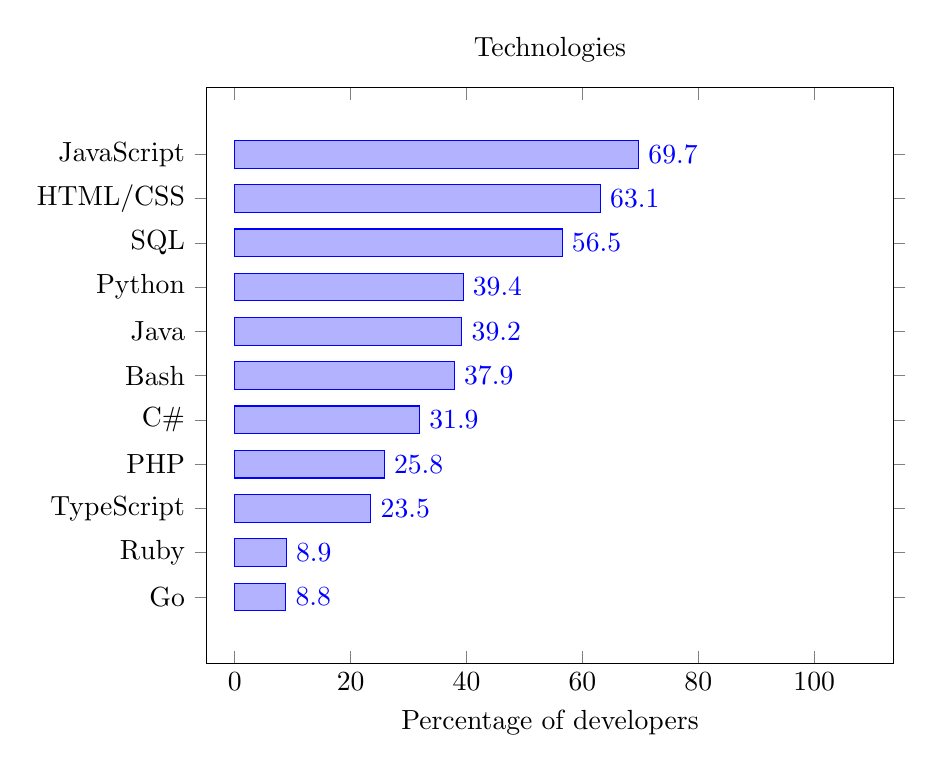
\begin{tikzpicture}
		\begin{axis}[
			xbar,
			title=Technologies,
			width=0.85\textwidth,
			xbar=0pt,
			xmax=100,
			enlargelimits=0.15,
			legend style={at={(0.5,-0.2)}, anchor=south,legend columns=-1},
			xlabel=Percentage of developers,
			symbolic y coords={
				Go,
				Ruby,
				TypeScript,
				PHP,
				C\#,
				Bash,
				Java,
				Python,
				SQL,
				HTML/CSS,
				JavaScript,
			},
			ytick=data,
			nodes near coords, 
			y tick label style={anchor=east},
			every axis plot/.append style={
				bar shift=0pt,
				fill
			  }
		]
		\addplot coordinates {
			(69.7,JavaScript)
			(63.1,HTML/CSS)
			(56.5,SQL)
			(39.4,Python)
			(39.2,Java)
			(37.9,Bash)
			(31.9,C\#)
			(25.8,PHP)
			(23.5,TypeScript)
			(8.9,Ruby)
			(8.8,Go)
		};
		\end{axis}
	\end{tikzpicture}
	%
	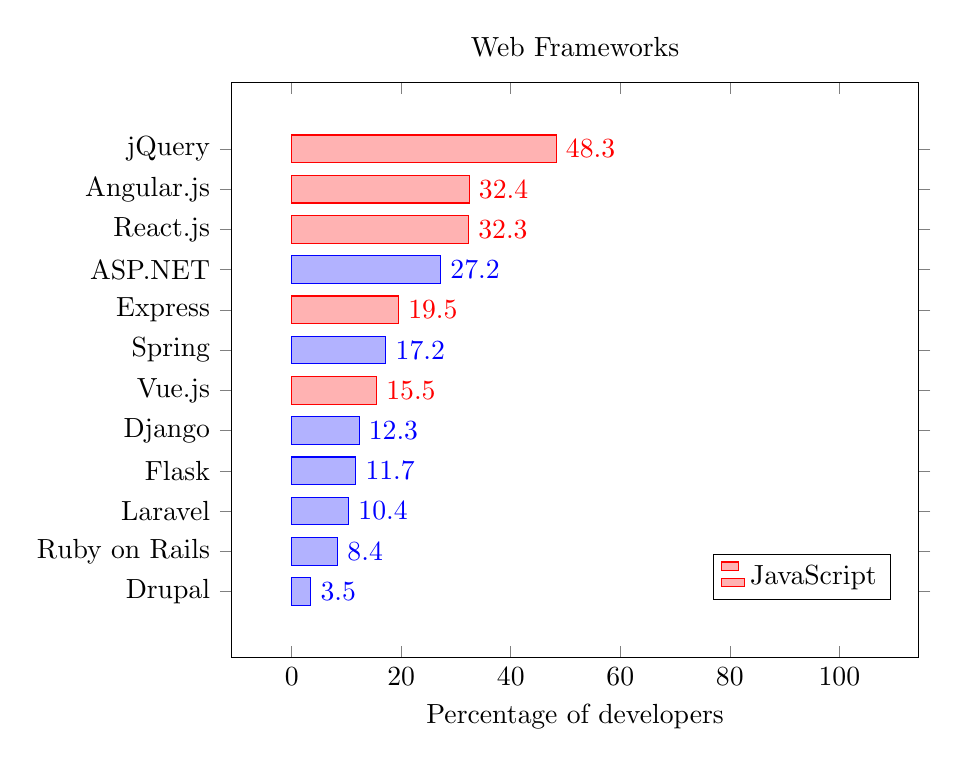
\begin{tikzpicture}
		\begin{axis}[
			xbar,
			title=Web Frameworks,
			width=0.85\textwidth,
			xbar=0pt,
			xmax=100,
			enlargelimits=0.15,
			legend style={at={(0.7,0.1)}, anchor=south west,legend columns=-1},
			xlabel=Percentage of developers,
			yticklabels={
				jQuery,
				Angular.js,
				React.js,
				ASP.NET,
				Express,
				Spring,
				Vue.js,
				Django,
				Flask,
				Laravel,
				Ruby on Rails,
				Drupal,
			},
			ytick={12, 11, ..., 1},
			nodes near coords, 
			y tick label style={anchor=east},
			every axis plot/.append style={
				bar shift=0pt,
				fill
			  }
		]

		\addplot coordinates {
			(27.2,9)
			(17.2,7)
			(12.3,5)
			(11.7,4)
			(10.4,3)
			(8.4,2)
			(3.5,1)
		};

		\addplot coordinates {
			(48.3,12)
			(32.4,11)
			(32.3,10)
			(19.5,8)
			(15.5,6)
		};

		\legend{,JavaScript}
		\end{axis}
	\end{tikzpicture}
	\caption[Conditional operators]{\textbf{Most Popular Technologies \& Frameworks 2019} - According to Stackoverflow's Developer Survey, JavaScript is the most commonly used programming language for 2019. 5 out of 12 of the most popular Web Frameworks are written in JavaScript.
	}
\end{figure}

\begin{figure}[tp]
	\centering
	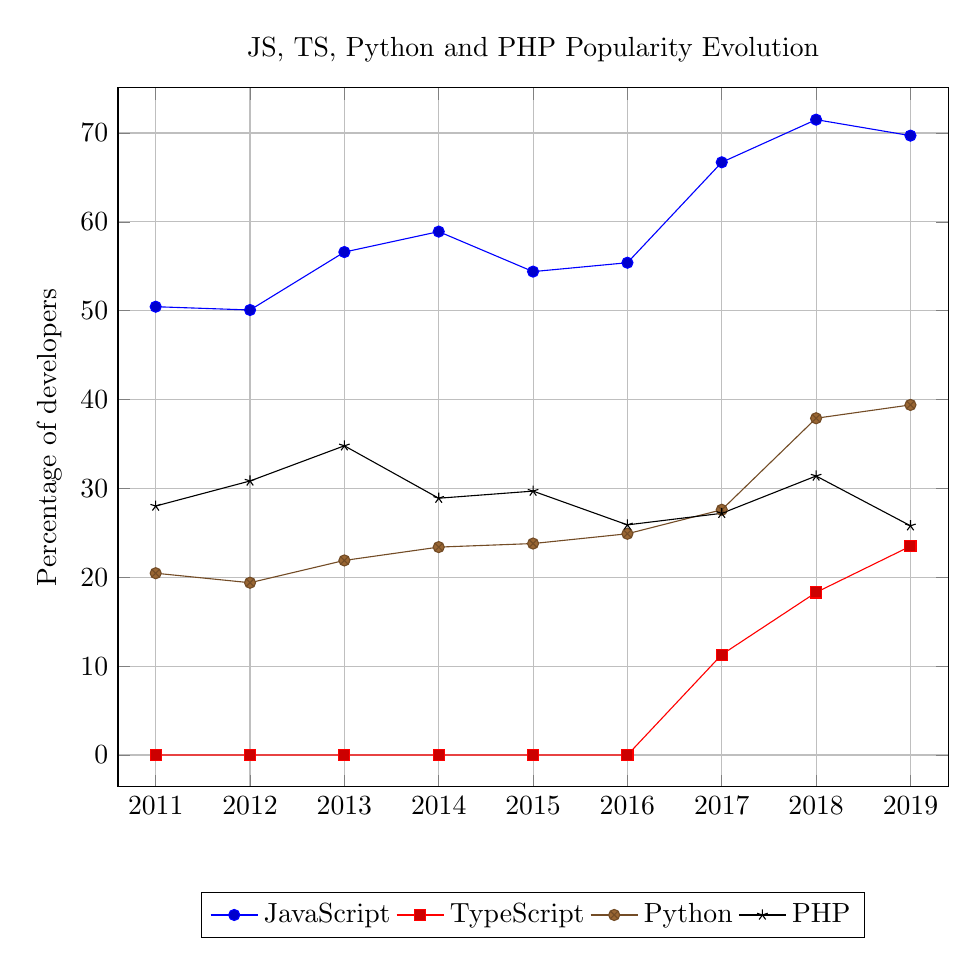
\begin{tikzpicture}
		\begin{axis}[
			width=1\textwidth,
			ylabel=Percentage of developers,
			title={JS, TS, Python and PHP Popularity Evolution},
			enlargelimits=0.05,
			legend style={at={(0.5,-0.15)},
				anchor=north,legend columns=-1},
			xticklabels={
				2011,
				2012,
				2013,
				2014,
				2015,
				2016,
				2017,
				2018,
				2019
			},
			xtick={0,...,8},
			grid=major,
		]

		% JavaScript
		\addplot coordinates {
			(0,50.45)
			(1,50.08)
			(2,56.60)
			(3,58.90)
			(4,54.40)
			(5,55.4)
			(6,66.7)
			(7,71.5)
			(8,69.7)
		};
		
		% TypeScript
		\addplot coordinates {
			(0,0)
			(1,0)
			(2,0)
			(3,0)
			(4,0)
			(5,0)
			(6,11.3)
			(7,18.3)
			(8,23.5)
		};
		
		% Python
		\addplot coordinates {
			(0,20.46)
			(1,19.39)
			(2,21.9)
			(3,23.4)
			(4,23.8)
			(5,24.9)
			(6,27.6)
			(7,37.9)
			(8,39.4)
		};

		% PHP
		\addplot coordinates {
			(0,28.02)
			(1,30.84)
			(2,34.8)
			(3,28.9)
			(4,29.7)
			(5,25.9)
			(6,27.2)
			(7,31.4)
			(8,25.8)
		};
		\legend{JavaScript,TypeScript,Python,PHP}
		\end{axis}
	\end{tikzpicture}
	\caption[Conditional operators]{\textbf{JS, TS, Python and PHP Popularity Evolution 2011 - 2019} - According to Stackoverflow's Developer Survey, for the seventh year in a row, JavaScript is the most commonly used programming language. While JavaScript's popularity remained constant for the last 3 years, TypeScript's popularity is increasing every year. There is no data for TypeScript before 2017.}
	\label{fig:background-programming-languages-evolution}
\end{figure}

\todo{Agregar tema serverless. Que NodeJS tiene el 75\% de los deploys}


\subsection{TypeCoercion}
\todo{Hablar de WTFS}
\todo{Aca incluir texto de what does it mean to be a JS Type}
\subsection{NPM Packages}
\todo{Agregar info de NPM by numbers! Cuantos downloads, cuantos packages, etc.}
\todo{https://snyk.io/blog/npm-passes-the-1-millionth-package-milestone-what-can-we-learn/}

\section{TypeScript}
\subsection{Declaration Files} \label{sec:declaration-files-background}
\subsection{Definitely Typedd}

\section{Jalangi} \label{sec:jalangi}